\documentclass{article}
\usepackage[utf8]{inputenc}
\usepackage[margin=3.5cm]{geometry}

% custom header/footer
\usepackage{fancyhdr}
\pagestyle{fancy}
\renewcommand{\headrulewidth}{0pt}
\fancyhf{}
\rfoot{\textsf{\thepage}}
\lfoot{\textsf{Suzie Brown}}

% miscellaneous formatting
\usepackage{xcolor}
\usepackage[font=small]{caption}
\usepackage{subcaption}
\usepackage{enumitem}
\usepackage{graphicx}

% maths
\usepackage{amsmath}
\usepackage{amssymb}
\usepackage{amsthm}
\usepackage{bbm}
\newtheorem{theorem}{Theorem}
\newtheorem{lemma}{Lemma}
\newtheorem{remark}{Remark}
\newcommand{\eqdist}{\overset{d}{=}}
\newcommand{\Prob}{\mathbb{P}}
\newcommand{\E}{\mathbb{E}}
\newcommand{\Et}{\mathbb{E}_t}
\newcommand{\V}{\operatorname{Var}}
\newcommand{\I}[1]{\mathbbm{1}_{\{#1\}}}
\newcommand{\1}[1]{\mathbbm{1}_{#1}}
\newcommand{\flnw}[1][i]{\lfloor N w_t^{(#1)} \rfloor}
\newcommand{\wbar}[2][t]{\bar{w}_{#1}^{(#2)}}
\newcommand{\Ht}{\mathcal{H}_t}
\newcommand{\midd}{\,\middle|\,} % big conditioning bar
\newcommand{\Cat}{\operatorname{Categorical}}
\newcommand{\Bin}{\operatorname{Binomial}}
\newcommand{\Mn}{\operatorname{Multinomial}}

%%% ANNOTATIONS
\usepackage{color}
\usepackage{xspace}
\newcommand{\seb}[1]{\xspace\textcolor{red}{#1}\xspace} 

\title{Convergence corollary for residual-multinomial resampling: a round-up of failed attempts}
\author{Suzie Brown}
\date{26 May 2021}

\begin{document}
\maketitle
\thispagestyle{fancy}


\section{Conditioning on the index set of deterministically-assigned offspring}

One way to separate the effects of the deterministic assignments from those of the stochastic (residual) assignments is to condition on which offspring will be assigned deterministically (resp. stochastically).\\

\begin{itemize}
\item $R:= N - \sum \flnw$ 
\item $r_i := \frac{1}{R} ( Nw_t^{(i)} - \flnw )$
\item Parent $i$ is deterministically assigned $\flnw$ offspring, for each $i$, and the remaining $R$ offspring are assigned to parents chosen independently $\sim \Cat(r_{1:N})$
\item Let $\mathcal{I} \subseteq [N]$ denote the index set of offspring that are assigned to the ``deterministic slots''
\item $|\mathcal{I}| = N-R = \sum \flnw$
\item $\mathcal{I} \mid w_t^{(1:N)}$ is uniform over the $\binom{N}{R}$ possible subsets of size $N-R$, due to the Standing Assumption
\item $a_t^{\mathcal{I}}$ and $a_t^{\mathcal{I}^c}$ are conditionally independent given $\mathcal{I}$, due to the Standing Assumption
\item The assumed bounds on $g_t$ imply almost surely $w_t^{(i)} \in [ \frac{1}{a^2 N}, \frac{a^2}{N} ]$, hence $\flnw \in [a^{-2}, a^2] $ and $|\mathcal{I}|= O(N)$
\end{itemize}
So...
\begin{equation}
\Prob[ a_t^{(1:N)} = a_{1:N} \mid \mathcal{H}_t ]
= \sum_{\mathcal{I}\subseteq[N]} \Prob[ \mathcal{I} \mid \mathcal{H}_t ]
        \, \Prob[ a_t^{\mathcal{I}} = a_{\mathcal{I}} \mid \mathcal{I}, \mathcal{H}_t ]
        \, \Prob[ a_t^{\mathcal{I}^c} = a_{\mathcal{I}^c} \mid \mathcal{I}, \mathcal{H}_t ]
\end{equation}
$\Prob[ \mathcal{I} \mid \mathcal{H}_t ]$ is not tractable, but will sum to one if the other terms can be bounded independently of $\mathcal{I}$.
\begin{equation}
\Prob[ a_t^{\mathcal{I}} = a_{\mathcal{I}} \mid \mathcal{I}, \mathcal{H}_t ]
\propto \left( \prod_{i=1}^N \I{ |\{ j \in \mathcal{I} : a_j =i \}| = \flnw } \right)
        \left( \prod_{i\in\mathcal{I}} q_{t-1}(X_t^{(a_i)}, X_{t-1}^{(i)} ) \right)
\end{equation}
Indicators ensure correct number of deterministic slots for each parent, $q$'s incorporate probability of particular parent-offspring assignment.
\begin{equation}
\Prob[ a_t^{\mathcal{I}^c} = a_{\mathcal{I}^c} \mid \mathcal{I}, \mathcal{H}_t ]
\propto \prod_{i\in\mathcal{I}^c} r_{a_i} q_{t-1}(X_t^{(a_i)}, X_{t-1}^{(i)} ) 
\end{equation}
$r$'s are the probabilities from the Categorical sampling of parents, $q$'s as above.




\section{Correct dominance of moments but with the wrong conditioning}

We set out to verify directly the main theorem condition in the case of residual-multinomial resampling. The desired relation was derived in the case where the conditioning was on the vector of weights, rather than on $\mathcal{H}_t$ (which takes into account information about one step in the future and can be exchanged for $\mathcal{F}_{t-1}$ due to conditional indpependence + tower rule) or $\mathcal{F}_{t-1}$ directly (which generally makes computing anything a bit impossible).\\

With residual-multinomial resampling, for each $i$
\begin{equation*}
\nu_t^{(i)} \mid w_t^{(1:N)}
\eqdist \flnw + X_i
\end{equation*}
where $X_i \sim \Bin(R, r_i)$. As usual, $R := N - \sum_{i=1}^N \flnw$ and $r_i := ( Nw_t^{(i)} - \flnw ) /R$.
\seb{If $R=0$ then $r_i = 0$ for all $i$ and the following calculations remain correct.}
We can therefore compute
\begin{align*}
\E [ (\nu_t^{(i)})_2 \mid w_t^{(1:N)} ]
&= \E\left[ (\flnw + X_i) (\flnw + X_i -1) \midd w_t^{(1:N)} \right] \\
&= (\flnw)_2 + 2\flnw E[ X_i \mid w_t^{(1:N)} ] + \E[ (X_i)_2 \mid w_t^{(1:N)} ] \\
&= (\flnw)_2 + 2\flnw R r_i + (R)_2 r_i^2
\end{align*}
using the moments of the Binomial distribution.
We also have
\begin{align*}
\E [ (\nu_t^{(i)})_3 \mid w_t^{(1:N)} ]
&= \E\left[ (\flnw + X_i) (\flnw + X_i -1) (\flnw + X_i -2) \midd w_t^{(1:N)} \right] \\
&= \flnw^3 + \flnw^2 \E[ 3X_i -3 \mid w_t^{(1:N)} ] \\
    &\hspace{1cm}+ \flnw 
        \E[ X_i(X_i-1) + X_i(X_i-2) + (X_i-1)(X_i-2) \mid w_t^{(1:N)} ] \\
    &\hspace{1cm}+ \E[ (X_i)_3 \mid w_t^{(1:N)} ] \\
&= \flnw^3 - 3\flnw^2 +3\flnw^2 \E[ X_i \mid w_t^{(1:N)} ] \\
    &\hspace{1cm}+ \flnw \E[ 3X_i^2 - 6X_i +2 \mid w_t^{(1:N)} ] 
        + E[(X_i)_3 \mid w_t^{(1:N)} ]\\
&= \left( \flnw^3 - 3\flnw^2 + 2\flnw \right)
        + 3 \left( \flnw^2 - \flnw \right) \E[ X_i \mid w_t^{(1:N)} ] \\
    &\hspace{1cm}+ 3 \flnw \E[ (X_i)_2 \mid w_t^{(1:N)} ] 
        + \E[ (X_i)_3 \mid w_t^{(1:N)} ] \\
&= (\flnw)_3 + 3(\flnw)_2 R r_i + 3\flnw (R)_2 r_i^2 + (R)_3 r_i^3 \\
&\leq \left( \flnw + R r_i \right) \left\{ (\flnw)_2 + 2\flnw R r_i 
        + (R)_2 r_i^2 \right\} \\
&= Nw_t^{(i)} \E[(\nu_t^{(i)})_2 \mid w_t^{(1:N)} ] \\
&\leq a^2 \E[(\nu_t^{(i)})_2 \mid w_t^{(1:N)} ] ,
\end{align*}
using the almost sure bound $w_t^{(i)} \leq a^2/N$.

...

\seb{To complete the proof we need to exchange the conditioning on $w_t^{(1:N)}$ for conditioning on $\mathcal{H}_t$ so we can then invoke the D-separation and tower property to get:}
\begin{equation*}
\frac{1}{(N)_3} \sum_{i=1}^N \Et [ (\nu_t^{(i)})_3 ]
\leq \frac{a^2}{N-2} \frac{1}{(N)_2} \sum_{i=1}^N \Et [ (\nu_t^{(i)})_2 ] .
\end{equation*}
Thus the main theorem condition is satisfied with $b_N = a^2/(N-2)$.
\seb{The $\varepsilon$ might want to get involved here as well once we switch the conditioning, coming from bounds on $q_t$ (which would then have to be included in the statement of this corollary).}




\section{Comparing coalescence rates between residual-multinomial and multinomial resampling}

The broad aim with this approach was to show a sort of $c_N$-ordering between residual-multinomial and multinomial resampling, conditional on the weight vector, which holds for any value of the weight vector and thus holds with any or no conditioning... Does it actually imply the same moment inequalities for the filtered expectations $\Et[\cdot]$, i.e. when the conditioning is $\mathcal{F}_{t-1}$? I'm not sure.\\

\subsection{Any $N$, one very large weight}

It has been suggested that we should expect the expected coalescence rate to be always lower in the case of residual-multinomial, but this has not yet been proven.
Some said that the proposed inequality could fail to hold when one or more weights are very large, causing a mega-coalescence to occur deterministically in the residual case, while multinomial resampling might chance to avoid the mega-coalescence.
As a not-very-compelling-but-somewhat-informative example, consider a scenario where one of the weights is $(N-1)/N$ or more.
\begin{equation*}
w_1 = \frac{N-1 +\gamma}{N}
\end{equation*}
for some $\gamma \in [0,1]$.
Thus the number of residual assignments is $R=1$ and the first residual is $r_1 = \gamma/1 = \gamma$.
\begin{align*}
\E[c_N^{res} \mid w_{1:N}] 
&= \frac{1}{(N)_2} \{ (N-1)_2 + (1)_2 \} \Prob[ \nu_1 = N-1 \mid w_{1:N} ]
        + \frac{1}{(N)_2} (N)_2 \Prob[ \nu_1 = N \mid w_{1:N} ] \\
&= \frac{(N-1)_2}{(N)_2} (1-\gamma)  + \gamma \\
&= 1 - \frac{2(1-\gamma)}{N} ,
\end{align*}
which, by the way, is equal to $2w_1 -1$.
Meanwhile under plain old multinomial resampling,
\begin{align*}
\E[c_N^{mn} \mid w_{1:N}] 
&= \sum_{i=1}^N w_i^2
= \left( \frac{N-1 +\gamma}{N} \right)^2 + \sum_{i=2}^N w_i^2 \\
&\geq \left( \frac{N-1 +\gamma}{N} \right)^2 
        + (N-1)\left( \frac{1-\gamma}{N(N-1)} \right)^2 \\
&= \frac{1}{N^2} \left\{ (N-1+\gamma)^2 + \frac{(1-\gamma)^2}{N-1} \right\} \\
&= \frac{1}{N^2} \left\{ N^2 - 2(1-\gamma) + \frac{N}{N-1}(1-\gamma)^2 \right\} \\
&\geq 1 - \frac{2(1-\gamma)}{N^2} \\
&\geq 1 - \frac{2(1-\gamma)}{N} .
\end{align*}
Thus, even in this frightening case of huge weights, we see that the coalescence rate is (considerably) higher with multinomial resampling than with residual-multinomial resampling.

Alas, it is still unclear whether this $c_N$-ordering holds for \emph{any} vector of weights, but this example might still our fears that it should fail when weights are large.


\subsection{Any $N$, lots of quite large weights}

One other special case we can construct in which $R=1$ (and so direct computation is not too difficult) is that where $N-1$ parents are deterministically assigned one offspring each:
\begin{equation*}
w_1 = \frac{\gamma}{N} , \qquad w_i \in \left[ \frac{1}{N}, \frac{2}{N} \right)
\end{equation*}
for each $i\neq 1$, where $\gamma \in [0,1)$.
Then, with residual-multinomial resampling,
\begin{align*}
\E[c_N^{res} \mid w_{1:N}] 
&= 0 \Prob[\nu_1 =1 \mid w_{1:N}] 
        + \sum_{i=2}^N \frac{2}{(N)_2} \Prob[\nu_i =2\mid w_{1:N}] \\
&= \frac{2}{(N)_2} \left( 1 - \Prob[\nu_1 =1 \mid w_{1:N}] \right) \\
&= \frac{2}{(N)_2} (1-\gamma)
\end{align*}
or, if you prefer, $=\frac{2}{N-1}((1/N) - w_1)$.

With plain old multinomial resampling,
\begin{align*}
\E[c_N^{mn} \mid w_{1:N}] 
&= \sum_{i=1}^N w_i^2
= \left( \frac{\gamma}{N} \right)^2 + \sum_{i=2}^N w_i^2 \\
&\geq \left( \frac{\gamma}{N} \right)^2 + (N-1) \left( \frac{1}{N} \right)^2 \\
&= \frac{1}{N^2} (\gamma^2 + N-1) \\
&= \frac{1}{(N)_2} \frac{N-1}{N}  (\gamma^2 + N-1) \\
&\geq \frac{1}{(N)_2} (\gamma^2 + N-2) \\
&\geq \frac{1}{(N)_2} (2 -2\gamma +N -4 ) \\
&\geq \frac{2}{(N)_2} (1-\gamma)
\end{align*}
whenever $N\geq 4$.
We see in this case also (though it was never in much doubt) that residual-multinomial resampling yields a lower expected coalescence rate than multinomial resampling. \\

We also have some results like the above that hold for \emph{any} weight vector, but so far only in the cases $N=2,3$ (and the limiting case $N=\infty$). These special cases are included below. Now we just need to show that the same inequality holds for $N=4,5,\dots$ --- ha ha.

\subsection{Case $N=2$}
\begin{lemma}
For all weight vectors $w_t^{(1:2)}$, 
$\E[c_2^m(t) |w_t^{(1:2)}] \geq \E[c_2^r(t) |w_t^{(1:2)}]$.
\end{lemma}

\begin{proof}
With only $N=2$ particles, the coalescence rate becomes
\begin{equation*}
\E[c_N(t) |w_t^{(1:2)}] = \frac{1}{(N)_2} \sum_{i=1}^{N} \E\left[ (\nu_t^{(i)})_2 |w_t^{(1:2)} \right] 
= \Prob[\nu_t^{(1)} = 0] + \Prob[\nu_t^{(1)} = 2].
\end{equation*}
For residual resampling,
\begin{equation*}
\E[c_2^r(t) |w_t^{(1:2)}] = \I{w_t^{(1)} \geq 1/2} (2w_t^{(1)} -1) + \I{w_t^{(1)} < 1/2} (2w_t^{(2)} -1)
\end{equation*}
And for multinomial resampling,
\begin{align*}
\E[c_2^m(t) |w_t^{(1:2)}] &= (w_t^{(1)})^2 + (w_t^{(2)})^2 \\
&= \I{w_t^{(1)} \geq 1/2} ((w_t^{(1)})^2 + (w_t^{(2)})^2) + \I{w_t^{(1)} < 1/2} ((w_t^{(1)})^2 + (w_t^{(2)})^2) \\
&\geq  \I{w_t^{(1)} \geq 1/2} (w_t^{(1)})^2 + \I{w_t^{(1)} < 1/2} (w_t^{(2)})^2
\end{align*}
Then since $(w_t^{(i)} -1)^2 = (w_t^{(i)})^2 -2w_t^{(i)} +1 \geq 0$, we have that $(w_t^{(i)})^2 \geq 2w_t^{(i)} -1$ and hence we conclude the proof.
\end{proof}

\begin{center}
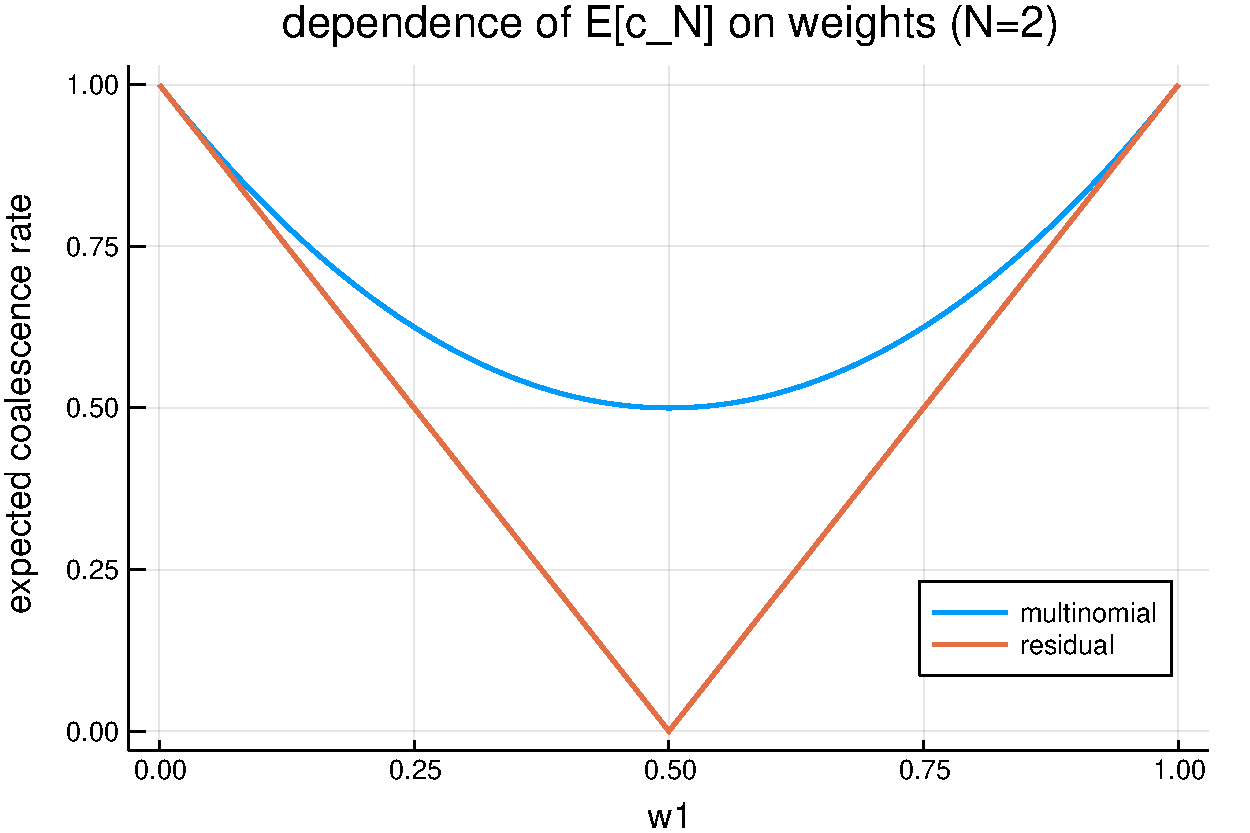
\includegraphics[width=0.8\textwidth]{plots/EcN_mn_res_N2.pdf}
\end{center}


\subsection{Case $N=3$}
Given a weight vector $(w_t^{(1)}, w_t^{(2)}, w_t^{(3)})$, let $w_{(1)} \geq w_{(2)} \geq w_{(3)}$ denote the weights sorted from high to low. 
With $N=3$ there are many more cases than with $N=2$, and these are described below, using the sorted weights.

In each case for the conditions on the sorted weights, the possible offspring count vectors (sorted in the same order as the weights) are listed, along with the probability of each (conditional on the given case). Finally, using these outcomes and associated probabilities, the conditional expectation of interest is calculated.\\

\begin{tabular}{ l | l | l | l | l }
Case & Weights & Offspring counts &  Conditional probabilities & $\E[c_2^r(t) | w_t^{(1:3)}]$ \\
\hline
(A) & $w_{(1)} = 1$ & $(3,0,0)$ & 1 & 1 \\
\hline
(B) & $2/3 < w_{(1)} < 1$ & $(3,0,0)$ & $3w_{(1)} - 2$ & $2w_{(1)} -1$\\
	&& $(2,1,0)$ & $3w_{(2)}$ & \\
	&& $(2,0,1)$  & $3w_{(3)}$ & \\
\hline
(C) & $w_{(1)}=2/3$ & $(2,1,0)$ & $3w_{(2)}$ & 1/3 \\
	&& $(2,0,1)$ & $3w_{(3)}$ & \\
\hline
(D1) & $1/3 < w_{(1)} < 2/3$ and & $(2,1,0)$ & $3w_{(1)} - 1$ & $1/3 - w_{(3)}$ \\
	& $1/3 \leq w_{(2)} < 2/3$ & $(1,2,0)$ & $3w_{(2)} -1$ & \\
	&& $(1,1,1)$ & $3w_{(3)}$  & \\
\hline
(D2) &  $1/3 < w_{(1)} < 2/3$ and & $(3,0,0)$ & $(3/2)^2 (w_{(1)} - 1/3)^2$ & $ (1/4) (3w_{(1)} - 1)(w_{(1)} + 1)$ \\
	& $w_{(2)} < 1/3$ & $(2,1,0)$ & $(3/2)^2 2(w_{(1)} - 1/3)w_{(2)}$ &\\
	&& $(2,0,1)$ & $(3/2)^2 2(w_{(1)} - 1/3)w_{(3)}$ &\\
	&& $(1,2,0)$ & $(3/2)^2 w_{(2)}^2$ &\\
	&& $(1,0,2)$ & $(3/2)^2 w_{(3)}^2$ &\\
	&& $(1,1,1)$ & $(3/2)^2 2w_{(2)} w_{(3)}$ &\\
\hline
(E) & $w_{(1)} = 1/3$ & $(1,1,1)$ & 1 & 0 \\
\end{tabular}

\vspace{0.6cm}

\begin{lemma}
For all weight vectors $w_t^{(1:3)}$, 
$\E[c_3^r(t) |w_t^{(1:3)}] \leq \E[c_3^m(t) |w_t^{(1:3)}]$.
\end{lemma}
\begin{proof}
We have the following expression in the case of residual resampling:
\begin{align*}
\E[c_3^r(t) |w_t^{(1:3)}] &= (2w_{(1)} -1) \I{2/3 \leq w_{(1)} \leq 1} \\
&\qquad + (1/3 - w_{(3)}) \I{1/3 \leq w_{(1)} < 2/3} \I{1/3 \leq w_{(2)} < 2/3} \\
&\qquad + (1/4)(3w_{(1)} -1)(w_{(1)} +1) \I{1/3 \leq w_{(1)} < 2/3} \I{w_{(2)} <1/3}
\end{align*}
compared to the following in the case of multinomial resampling:
\begin{align*}
\E[c_3^m(t) |w_t^{(1:3)}] &= w_{(1)}^2 + w_{(2)}^2 + w_{(3)}^2 \\
&= (w_{(1)}^2 + w_{(2)}^2 + w_{(3)}^2) \I{2/3 \leq w_{(1)} \leq 1} \\
&\qquad + (w_{(1)}^2 + w_{(2)}^2 + w_{(3)}^2) \I{1/3 \leq w_{(1)} < 2/3} \I{1/3 \leq w_{(2)} < 2/3} \\
&\qquad + (w_{(1)}^2 + w_{(2)}^2 + w_{(3)}^2) \I{1/3 \leq w_{(1)} < 2/3} \I{w_{(2)} <1/3}.
\end{align*}
Hence it suffices to show the following:
\begin{enumerate}[label=(\roman*)]
\item $(2w_{(1)} -1) \leq (w_{(1)}^2 + w_{(2)}^2 + w_{(3)}^2)$
\item $ (1/3 - w_{(3)}) \leq (w_{(1)}^2 + w_{(2)}^2 + w_{(3)}^2)$
\item $ (1/4)(3w_{(1)} -1)(w_{(1)} +1) \leq (w_{(1)}^2 + w_{(2)}^2 + w_{(3)}^2)$\\
\end{enumerate}
First consider (ii). Since $w_{(3)}$ is defined as the smallest of the three weights, we know that $w_{(3)} \in [0,1/3]$. Meanwhile, the RHS is the sum of the squared weights, which is always between 1/3 and 1. Therefore (ii) is true.\\[7pt]
Now let us consider (i). We have the identity $(w_{(1)} -1)^2 = w_{(1)}^2 -2w_{(1)} +1$, which implies that $w_{(1)}^2 \geq 2_w{(1)} - 1$. Since $w_{(2)}^2 + w_{(3)}^2 \geq 0$ we can therefore conclude that (i) is true.\\[7pt]
Finally consider (iii). In this case it is sufficient to show that $(1/4)(3w_{(1)} -1)(w_{(1)} +1) \leq w_{(1)}^2$. Note that
\begin{align*}
& w_{(1)}^2 - \frac{1}{4}(3w_{(1)} -1)(w_{(1)} +1) \\
& = \frac{1}{4} w_{(1)}^2- \frac{1}{2} w_{(1)} + \frac{1}{4} \\
& = \frac{1}{4} (w_{(1)} -1)^2 \geq 0.
\end{align*}
Therefore (iii) is also true, concluding the proof.
\end{proof}

\begin{figure}
	\centering
	\begin{subfigure}{\textwidth}
		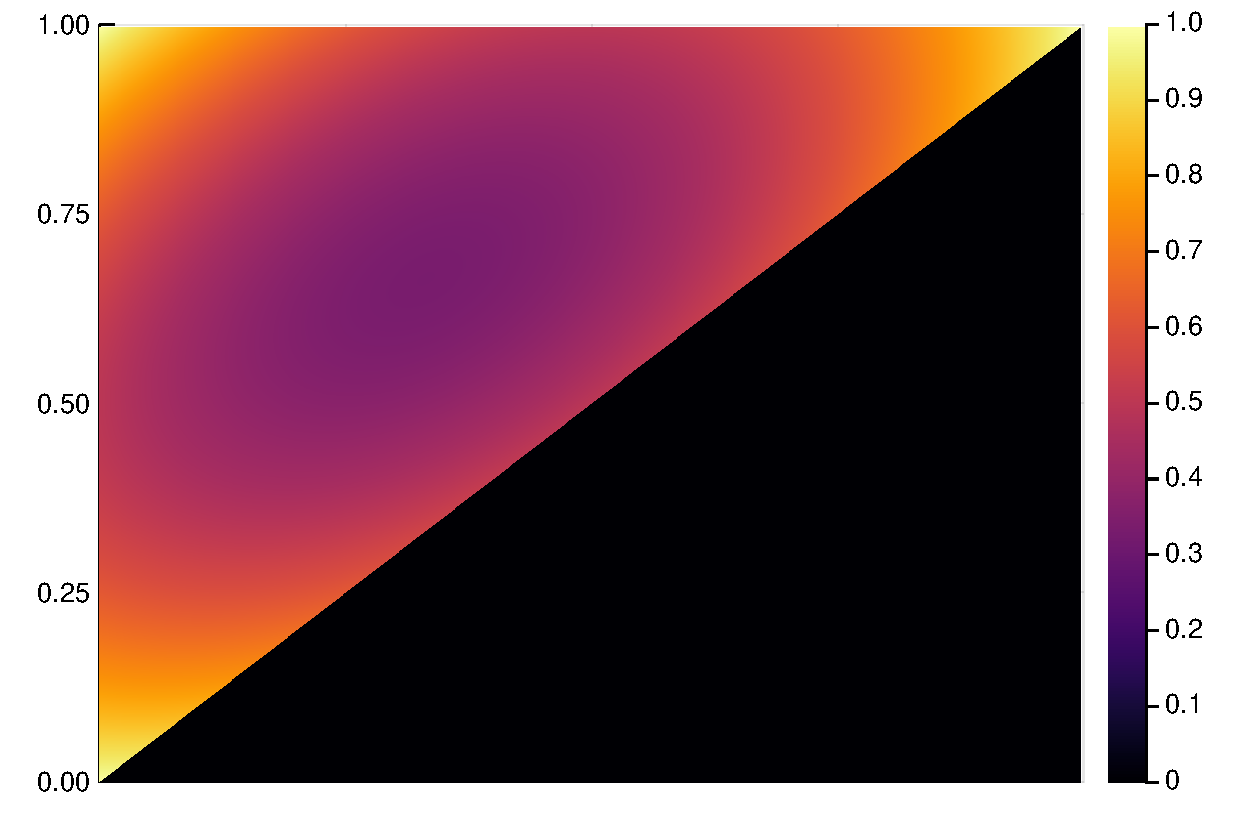
\includegraphics[width=0.5\textwidth]{plots/EcN_mn_N3_heatmap.pdf}
		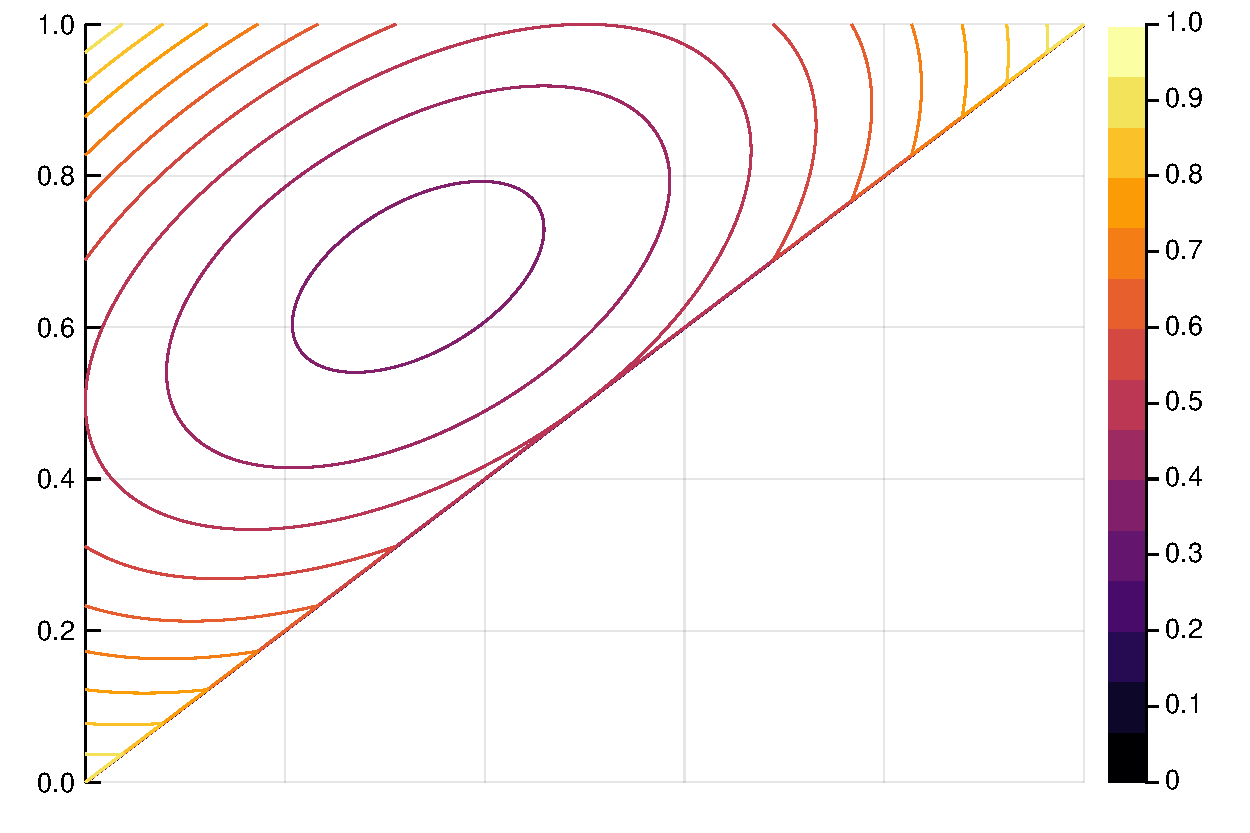
\includegraphics[width=0.5\textwidth]{plots/EcN_mn_N3_contour.pdf}
	\caption{Expected coalescence rate with multinomial resampling ($N=3$)}
	\end{subfigure}
	\begin{subfigure}{\textwidth}
		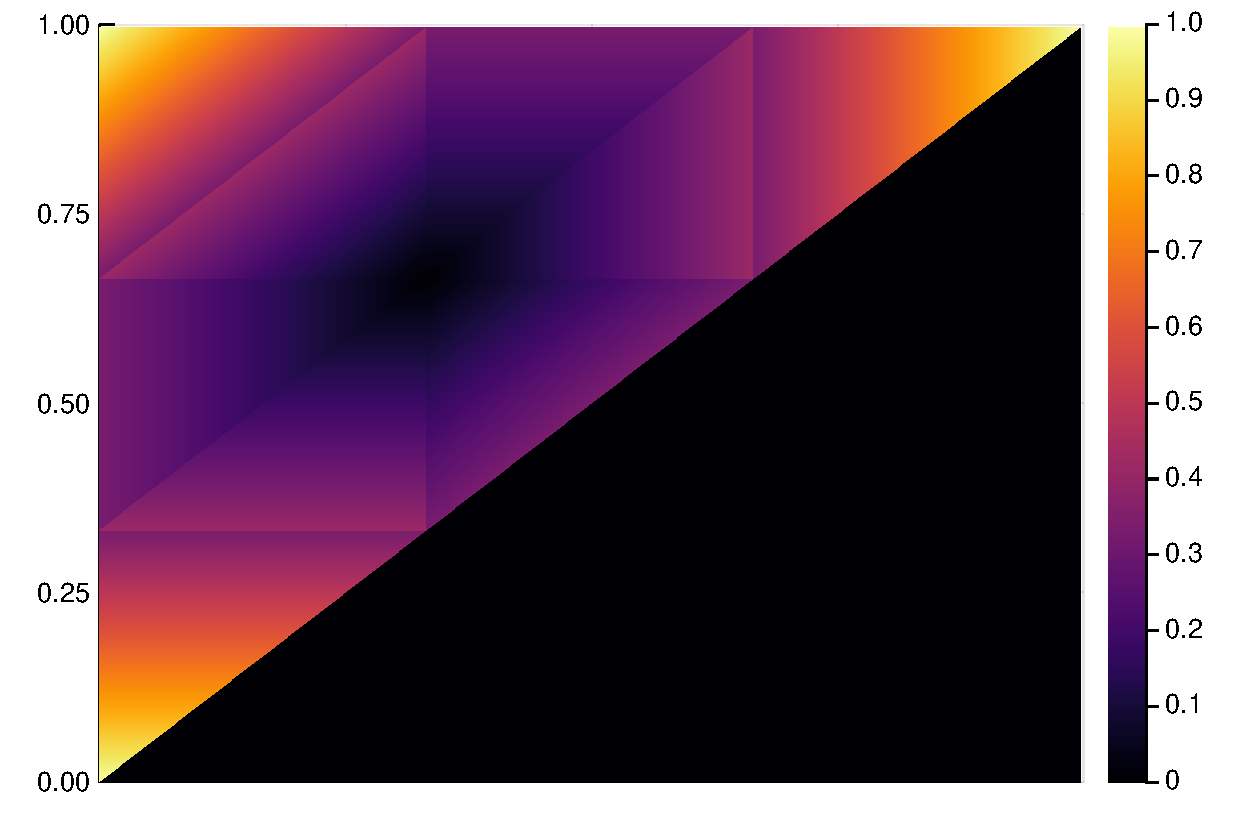
\includegraphics[width=0.5\textwidth]{plots/EcN_res_N3_heatmap.pdf}
		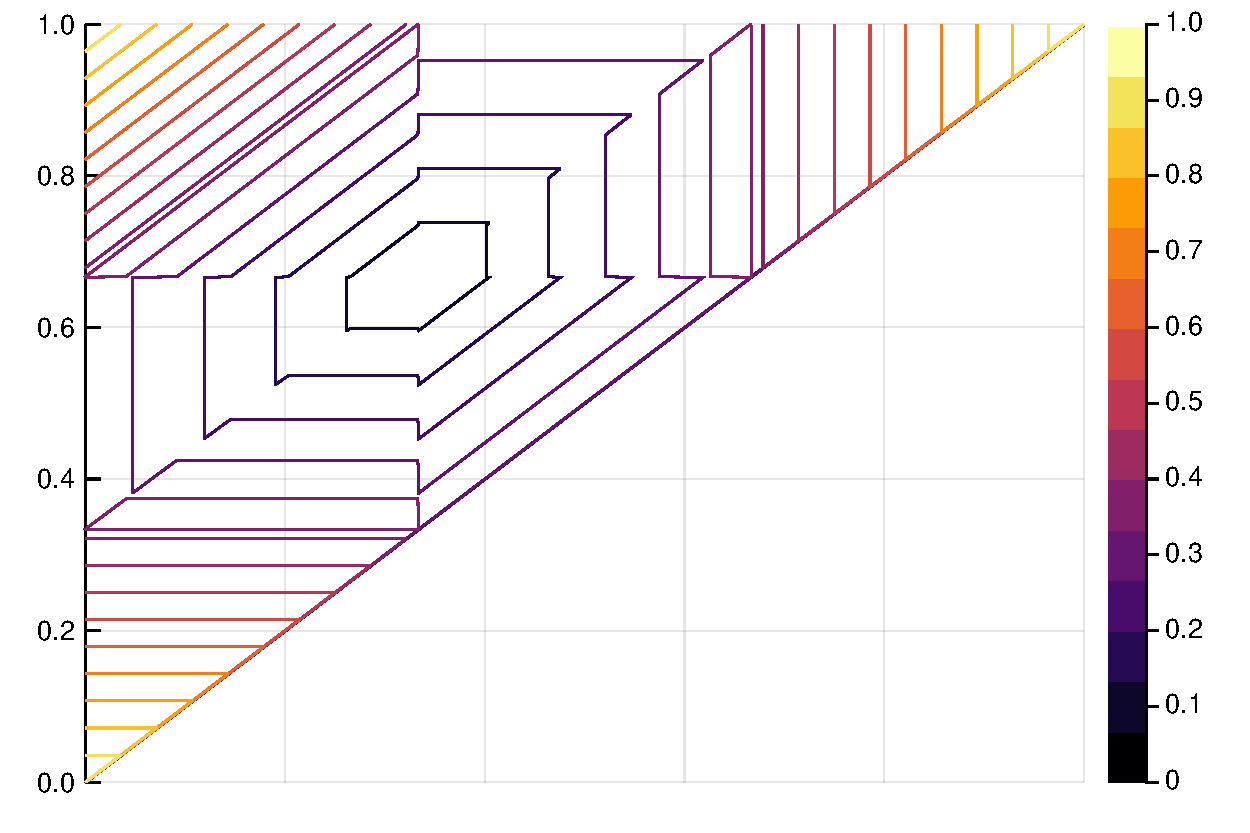
\includegraphics[width=0.5\textwidth]{plots/EcN_res_N3_contour.pdf}
	\caption{Expected coalescence rate with residual resampling ($N=3$)}
	\end{subfigure}
	\begin{subfigure}{\textwidth}
		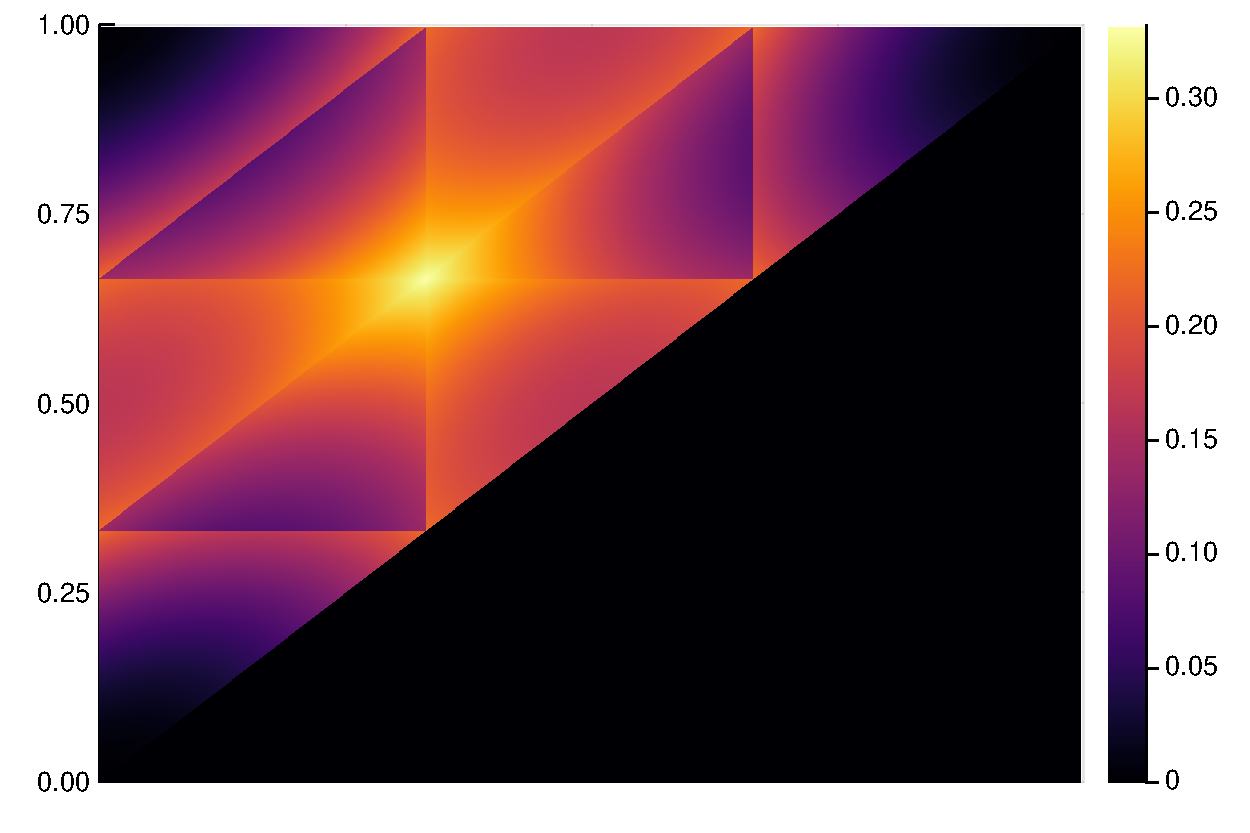
\includegraphics[width=0.5\textwidth]{plots/EcN_mn_res_diff_N3_heatmap.pdf}
		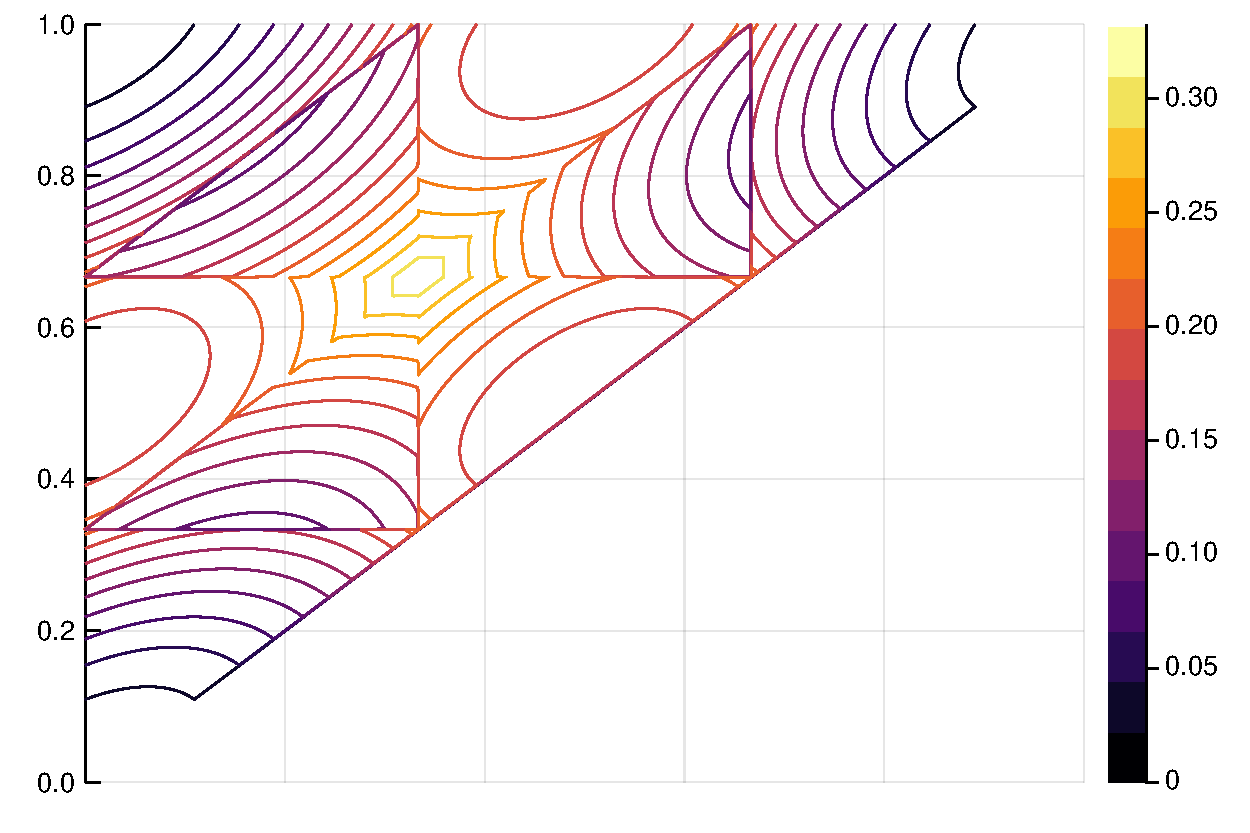
\includegraphics[width=0.5\textwidth]{plots/EcN_mn_res_diff_N3_contour.pdf}
	\caption{Difference between expected coalescence rate with multinomial or residual resampling ($N=3$)}
	\end{subfigure}
\end{figure}

\begin{remark}
Examining the table, we can see that the function $\E[c_3^r(t) |w_t^{(1:3)}]$ is continuous in $w_{(1)}$. However, the plot clearly shows discontinuities. These occur at the boundaries between different orderings when we sort the weights from high to low.
\end{remark}







\section{Coupling between multinomial and residual-multinomial resampling}

The idea was to find a coupling between the multinomial/categorical distribution induced by multinomial resampling and the multinomial/categorical distribution induced by the stochastic part of residual resampling. It didn't work because these distributions are parametrised by a different weight vector in each case: $w_{1:N}$ in the multinomial scheme, and $r_{1:N}$ in the residual-multinomial scheme. So it was not possible to prove any kind of dominance using the coupling method.




\section{Direct computation of the filtered moments}

The hope with this attempt was to show directly, without any intermediate conditioning that the filtered expectations (being the objects we are actually interesting), the desired ordering between residual-multinomial and multinomial resampling. Up to now I have been unable to show that the expression derived below for $\E[c^r_N(t) |\mathcal{F}_{t-1}]$ is bounded by the corresponding quantity for multinomial resampling. 

Even if this were shown, we'd still need the opposite inequality for the third factorial moments. Then the bounds obtained in the multinomial resampling corollary could be applied for residual-multinomial too. 

It seems to me that we should not really expect opposite inequalities to hold for second versus third moments, since we know (or at least feel) that residual-multinomial gives ``more concentrated'' offspring counts, so there could be a convex ordering which would imply the inequality the same way around for both second and third factorial monents (since both $(\nu)_2$ and $(\nu)_3$ are convex functions on $\mathbb{N}$.\\




The offspring counts are sampled according to:
\begin{align*}
& \nu_t^{(i)} = \lfloor N w_t^{(i)} \rfloor + X_i \\
& X_i \sim \Mn (N-k, (\wbar{1}, \dots, \wbar{N}))
\end{align*}
where $k := \sum_{i=1}^N \lfloor N w_t^{(i)} \rfloor$ is the number of offspring assigned deterministically, and $\wbar{i} := \frac{Nw_t^{(i)} - \lfloor N w_t^{(i)} \rfloor}{N - k}$ are the residual weights. Let us also define the residuals $r_i := Nw_t^{(i)} - \lfloor N w_t^{(i)} \rfloor$. So $\sum_{i=1}^N r_i = N-k$.

The coalescence rate is defined as
\begin{equation*}
c_N(t) := \frac{1}{(N)_2} \sum_{i=1}^{N} (\nu_t^{(i)})_2.
\end{equation*}
We will use $c_N^m(t)$ and $c_N^r(t)$ to denote the coalescence rates with multinomial and residual resampling respectively.
The expectation then comes out as
\begin{align*}
\E[(\nu_t^{(i)})_2 |\mathcal{F}_{t-1}] &= \E[(\nu_t^{(i)})^2 |\mathcal{F}_{t-1}] - \E[\nu_t^{(i)} |\mathcal{F}_{t-1}] \\
&= \E[\lfloor Nw_t^{(i)} \rfloor^2 |\mathcal{F}_{t-1}] + 2 \E[\lfloor Nw_t^{(i)} \rfloor r_i |\mathcal{F}_{t-1}] + \E\left[ r_i \left(1 - \frac{r_i}{N-k} + r_i \right) |\mathcal{F}_{t-1} \right] - \E[Nw_t^{(i)} |\mathcal{F}_{t-1}] \\
&=\E[ \lfloor Nw_t^{(i)} \rfloor^2 |\mathcal{F}_{t-1}] - \E[ \lfloor Nw_t^{(i)} \rfloor |\mathcal{F}_{t-1}] + 2 \E[ \lfloor Nw_t^{(i)} \rfloor r_i |\mathcal{F}_{t-1}] + \E\left[ r_i^2 \left(1- \frac{1}{N-k} \right) |\mathcal{F}_{t-1}\right] \\
&= \E[ (Nw_t^{(i)})^2 |\mathcal{F}_{t-1}] - \E[ \lfloor Nw_t^{(i)} \rfloor |\mathcal{F}_{t-1}] - \E\left[ \frac{r_i^2}{N-k} |\mathcal{F}_{t-1} \right]
\end{align*}
so we get
\begin{align}
\E[c^r_N(t) |\mathcal{F}_{t-1}] &=  \frac{1}{(N)_2}  \sum_{i=1}^{N} \E[(\nu_t^{(i)})_2 |\mathcal{F}_{t-1} ]\notag\\
&= \frac{N}{N-1} \sum_{i=1}^{N} \E[(w_t^{(i)})^2 |\mathcal{F}_{t-1}] - \frac{1}{(N)_2} \sum_{i=1}^{N} \E\left[ \frac{r_i^2}{N-k} |\mathcal{F}_{t-1} \right] - \frac{1}{(N)_2} \E[k |\mathcal{F}_{t-1}] \notag\\
&= \E[c^{m}_N(t) |\mathcal{F}_{t-1}] \left( 1 + \frac{1}{N-1} \right) - \frac{1}{(N)_2}  \E\left[ \frac{\sum_{i=1}^{N} (Nw_t^{(i)} - \lfloor Nw_t^{(i)}\rfloor)^2}{\sum_{j=1}^{N} (Nw_t^{(j)} - \lfloor Nw_t^{(j)}\rfloor)} \middle|\mathcal{F}_{t-1} \right] \notag\\
&\qquad -\frac{1}{(N)_2} \E \left[ \sum_{i=1}^{N} \lfloor Nw_t^{(i)}\rfloor \middle|\mathcal{F}_{t-1} \right]
\label{eq:cNt_1}
\end{align}
\textbf{Sanity check:}\\
When the weights are all equal (almost surely), $w_t^{(i)} \equiv 1/N$, we should have $\E[c^r_N(t) |\mathcal{F}_{t-1}] = 0$ since each particle will have exactly one offspring so it is impossible for any lineages to coalesce. In this case we have $\E[c^{m}_N(t) |\mathcal{F}_{t-1}] = \sum_{i=1}^{N} \E[(w_t^{(i)})^2 |\mathcal{F}_{t-1}] = 1/N$ for multinomial resampling. We also have that $Nw_t^{(i)} \equiv \lfloor Nw_t^{(i)} \rfloor \equiv 1$ and hence $r_i = 0$ and $k=N$. Thus the RHS comes out as
\begin{equation*}
\frac{1}{N}\frac{N}{N-1} - 0 - \frac{1}{(N)_2} N = \frac{1}{N-1} - \frac{1}{N-1} = 0
\end{equation*}
as expected.\\

We can write it in a different form by combining the second and third terms of \eqref{eq:cNt_1}:
\begin{align*}
&- \frac{1}{(N)_2}  \E\left[ \frac{\sum_{i=1}^{N} (Nw_t^{(i)} - \lfloor Nw_t^{(i)}\rfloor)^2}{\sum_{j=1}^{N} (Nw_t^{(j)} - \lfloor Nw_t^{(j)}\rfloor)} |\mathcal{F}_{t-1} \right] 
-\frac{1}{(N)_2} \E \left[ \sum_{k=1}^{N} \lfloor Nw_t^{(k)}\rfloor \middle|\mathcal{F}_{t-1} \right] \\
&=: - \frac{1}{(N)_2} \E[A |\mathcal{F}_{t-1}]
\end{align*}
Then
\begin{align*}
A &=
 \frac{\sum_{i=1}^{N} (Nw_t^{(i)} - \lfloor Nw_t^{(i)}\rfloor)^2}{\sum_{j=1}^{N} (Nw_t^{(j)} - \lfloor Nw_t^{(j)}\rfloor)} 
+ \sum_{k=1}^{N} \lfloor Nw_t^{(k)}\rfloor \\
&= \frac{\sum_{i=1}^{N} (Nw_t^{(i)} - \lfloor Nw_t^{(i)}\rfloor)^2 + \sum_{i=1}^N\sum_{k=1}^N \lfloor Nw_t^{(k)} \rfloor (Nw_t^{(i)}- \lfloor Nw_t^{(i)} \rfloor)}{\sum_{j=1}^{N} (Nw_t^{(j)} - \lfloor Nw_t^{(j)}\rfloor)} \\
&=: \frac{A^\prime}{\sum_{j=1}^{N} (Nw_t^{(j)} - \lfloor Nw_t^{(j)}\rfloor)} 
\end{align*}
Then
\begin{align*}
A^\prime &=
\sum_{i=1}^{N} (Nw_t^{(i)} - \lfloor Nw_t^{(i)}\rfloor)^2 + \sum_{i=1}^N\sum_{k=1}^N \lfloor Nw_t^{(k)} \rfloor (Nw_t^{(i)}- \lfloor Nw_t^{(i)} \rfloor)\\
&= \sum_{i=1}^{N} \left\{ \left(Nw_t^{(i)} - \lfloor Nw_t^{(i)}\rfloor \right)^2 + \lfloor Nw_t^{(i)} \rfloor \left(Nw_t^{(i)} - \lfloor Nw_t^{(i)}\rfloor \right)
+ \sum_{k\neq i} \lfloor Nw_t^{(k)} \rfloor \left(Nw_t^{(i)} - \lfloor Nw_t^{(i)}\rfloor \right) \right\}\\
&= \sum_{i=1}^{N} \left\{ (Nw_t^{(i)})^2 - Nw_t^{(i)} \lfloor Nw_t^{(i)} \rfloor 
+ \sum_{k\neq i} \lfloor Nw_t^{(k)} \rfloor \left(Nw_t^{(i)} - \lfloor Nw_t^{(i)}\rfloor \right) \right\}\\
 &= \sum_{i=1}^{N} \left\{ \left(Nw_t^{(i)} - \lfloor Nw_t^{(i)} \rfloor \right) \left( Nw_t^{(i)} + \sum_{k\neq i} \lfloor Nw_t^{(k)} \rfloor \right) \right\}
\end{align*}
So we have
\begin{align*}
\E[c^r_N(t) |\mathcal{F}_{t-1}] &=  \E[c^{m}_N(t) |\mathcal{F}_{t-1}] \left( 1 + \frac{1}{N-1} \right) \\
&\qquad- \frac{1}{(N)_2}  \E\left[ \frac{\sum_{i=1}^{N} \left(Nw_t^{(i)} - \lfloor Nw_t^{(i)} \rfloor \right) \left( Nw_t^{(i)} + \sum_{k\neq i} \lfloor Nw_t^{(k)} \rfloor \right) }{\sum_{j=1}^{N} \left(Nw_t^{(j)} - \lfloor Nw_t^{(j)}\rfloor\right)} \middle|\mathcal{F}_{t-1} \right] .
\end{align*}



\end{document}